\documentclass[12pt,a4paper]{article}
\usepackage{iftex}
\ifPDFTeX
  \usepackage[T2A]{fontenc}
  \usepackage[utf8]{inputenc}
\else
  \usepackage{fontspec}
  \setmainfont[BoldFont=DejaVuSerif-Bold.ttf,
    ItalicFont=DejaVuSerif-Italic.ttf,
    BoldItalicFont=DejaVuSerif-BoldItalic.ttf]{DejaVuSerif.ttf}
  \setmonofont[BoldFont=DejaVuSansMono-Bold.ttf,
    ItalicFont=DejaVuSansMono-Oblique.ttf,
    BoldItalicFont=DejaVuSansMono-BoldOblique.ttf]{DejaVuSansMono.ttf}
\fi
\usepackage[russian]{babel}
\usepackage[left=25mm,right=15mm,top=20mm,bottom=20mm]{geometry}
\usepackage{indentfirst}
\usepackage{graphicx}
\usepackage{float}
\graphicspath{{figures/}}
\setlength{\parindent}{1.25cm}
\setlength{\parskip}{2pt}
\emergencystretch=2em

\begin{document}
\begin{titlepage}
\begin{center}
\textbf{Наименование образовательной организации}\\[1mm]
\underline{\hspace{125mm}}\\[3mm]
Кафедра \underline{\hspace{95mm}}

\vfill
{\Large\bfseries ОТЧЁТ ПО КУРСОВОЙ РАБОТЕ}\\[6mm]
{\large по дисциплине \underline{\hspace{70mm}}}\\[7mm]
{\large\bfseries Программа автоматической синхронизации файлов в двух каталогах на разных компьютерах}
\end{center}
\vfill
\begin{flushright}
\begin{tabular}{ll}
Выполнил студент: & \underline{\hspace{55mm}}\\[4mm]
Группа: & \underline{\hspace{55mm}}\\[4mm]
Проверил: & \underline{\hspace{55mm}}
\end{tabular}
\end{flushright}
\vfill
\begin{center}
\underline{\hspace{50mm}} --- 2026
\end{center}
\end{titlepage}

\tableofcontents
\newpage
\section{Функциональная спецификация}
\subsection{Назначение и среда работы}

Программа предназначена для автоматической двусторонней синхронизации файлов между двумя каталогами на разных компьютерах. На каждом компьютере запускается экземпляр программы. Экземпляры взаимодействуют непосредственно по сети с помощью TCP-сокетов; выделенный сервер и СУБД не требуются. Для запуска необходима Java версии 17 или новее.

\subsection{Исходные данные и управление}

Пользователь указывает существующий локальный каталог, адрес второго компьютера, локальный TCP-порт, порт второго экземпляра и интервал проверки в секундах. Настройки вводятся в графическом окне либо передаются параметрами командной строки. После запуска каждый экземпляр принимает входящие соединения и периодически инициирует обмен со вторым экземпляром. Доступна команда немедленной проверки. При недоступности узла следующая попытка выполняется через заданный интервал.

\subsection{Правила обработки файлов}

Программа рекурсивно формирует список обычных файлов в каталоге. Для каждого файла сохраняются его относительный путь, размер и хэш SHA-256. Экземпляры обмениваются списками и сравнивают файлы по относительным путям.

\begin{itemize}
  \item Файл, присутствующий только в одном каталоге, передаётся в другой каталог с сохранением относительного пути.
  \item Файлы с одинаковым путём и одинаковым содержимым повторно не копируются.
  \item При одинаковом пути и различном содержимом возникает конфликт: обе версии сохраняются, а сообщение с путём и хэшами записывается в журнал.
  \item Получаемые данные сначала записываются во временный файл и проверяются по размеру и хэшу. Существующий файл не перезаписывается.
\end{itemize}

Удаления между каталогами не распространяются: отсутствующий файл при следующей проверке копируется снова. Пустые каталоги отдельно не передаются. Символические ссылки не синхронизируются. Каталог \texttt{.filesynchronizer-tmp} в корне выбранного каталога зарезервирован для временных файлов и исключён из обмена; собственный файл журнала также исключается. Имена с обратной косой чертой или двоеточием не поддерживаются, поскольку такие имена несовместимы с файловыми системами разных ОС.

\subsection{Журнал и сообщения об ошибках}

В текстовый журнал записываются запуск и остановка сервера, адреса подключившихся клиентов, сведения о переданных файлах, результаты проверок, конфликты и ошибки. В графическом режиме эти сообщения одновременно отображаются в окне. Ошибки настройки выводятся пользователю. При разрыве соединения незавершённый файл не устанавливается как результат, а обмен повторяется при следующей проверке.

\subsection{Ограничения и требования к реализации}

Соединение не шифруется и не проверяет личность удалённой стороны, поэтому программа рассчитана на доверенную сеть. Реализация разделена на модель, представление, контроллер, сетевую подсистему и вспомогательные средства. Приложение и тесты используют стандартную библиотеку Java. Проект собирается Maven; сборка компилирует программу, выполняет тесты модели и сетевого взаимодействия и создаёт JAR-файлы программы и тестов.


\section{Руководство пользователя}
\subsection{Подготовка и сборка}

Установите JDK версии 17 или новее и Maven версии 3.8 или новее. Откройте командную строку в каталоге проекта \texttt{FileSynchronizer} и выполните:
\begin{verbatim}
mvn clean package
\end{verbatim}
Maven компилирует исходный код, выполняет тесты и формирует два архива в каталоге \texttt{target}: исполняемый \texttt{FileSynchronizer-1.0.jar} и архив тестов \texttt{FileSynchronizer-1.0-tests.jar}. Отдельно тесты запускаются командой \texttt{mvn test}, очистка --- командой \texttt{mvn clean}. Для сетевого теста должны быть разрешены локальные соединения с адресом \texttt{127.0.0.1}.

\subsection{Запуск с графическим интерфейсом}

На каждом компьютере выполните команду:
\begin{verbatim}
java -jar target/FileSynchronizer-1.0.jar
\end{verbatim}
Откроется окно, показанное на рисунке~\ref{fig:main}. В поле «Каталог» задайте существующий каталог или выберите его кнопкой «Обзор». Далее введите адрес другого компьютера, свой локальный порт, порт другого экземпляра и интервал в секундах.

\begin{figure}[H]
\centering
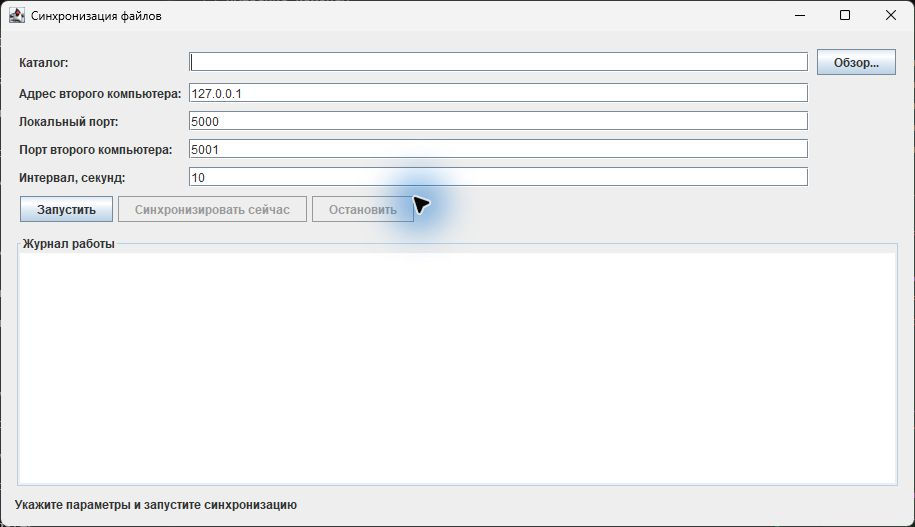
\includegraphics[width=\linewidth]{main-window.png}
\caption{Главное окно перед настройкой}
\label{fig:main}
\end{figure}

Например, первому экземпляру можно назначить локальный порт 5000 и удалённый порт 5001, второму --- локальный порт 5001 и удалённый порт 5000. При проверке на одном компьютере оба экземпляра используют адрес \texttt{127.0.0.1}, но разные каталоги и порты. На двух компьютерах вместо этого адреса вводится сетевой адрес партнёра. При необходимости пользователь разрешает входящие TCP-соединения на выбранных портах в брандмауэре.

Нажмите «Запустить» в обоих экземплярах. Если второй ещё не запущен, первый может вывести ошибку соединения и повторит попытку позже. Кнопка «Синхронизировать сейчас» инициирует дополнительную проверку. Результаты отображаются в журнале; пример передачи файлов и обнаружения конфликта приведён на рисунке~\ref{fig:result}. Для завершения нажмите «Остановить» или закройте окно.

\begin{figure}[H]
\centering
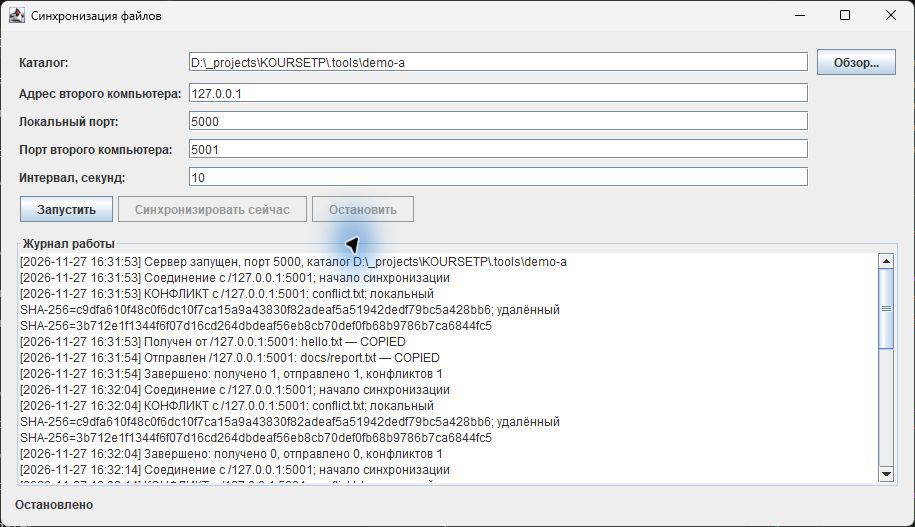
\includegraphics[width=\linewidth]{synchronization.png}
\caption{Журнал после обмена: полученный и отправленный файлы, сообщение о конфликте}
\label{fig:result}
\end{figure}

По умолчанию журнал находится в файле \texttt{logs/sync-<порт>.log} относительно текущего рабочего каталога. При конфликте остановите синхронизацию, сравните версии и вручную оставьте нужное содержимое в обоих каталогах. Не удаляйте файл только на одной стороне: программа скопирует его обратно.

\subsection{Работа из командной строки}

Кроме графического интерфейса предусмотрен режим без окна. Пример для первого компьютера:
\begin{verbatim}
java -jar target/FileSynchronizer-1.0.jar
  --directory "C:\sync-a" --local-port 5000
  --peer 192.168.1.20 --peer-port 5001 --interval 10
\end{verbatim}
Здесь переносы строк приведены для наглядности; команду следует ввести одной строкой. На втором компьютере нужно указать свой каталог, локальный порт 5001, адрес первого компьютера и порт 5000. Параметр \texttt{--log} задаёт путь к журналу; \texttt{--once} выполняет одну попытку и завершает процесс. Справка доступна с параметром \texttt{--help}, постоянная работа завершается сочетанием Ctrl+C.

\section{Архитектура программы}

Архитектура разделяет представление и обработку команд, модель, контроллер и сетевую подсистему. Каждый экземпляр содержит и клиент, и сервер. Общая схема показана на рисунке~\ref{fig:architecture}.

\begin{figure}[H]
\centering
\setlength{\unitlength}{1mm}
\begin{picture}(164,75)
\put(0,48){\framebox(37,20){\parbox{35mm}{\centering\small Представление\\Swing / CLI}}}
\put(43,48){\framebox(37,20){\parbox{34mm}{\centering Контроллер\\расписание}}}
\put(86,48){\framebox(37,20){\parbox{34mm}{\centering Сеть\\клиент / сервер}}}
\put(129,48){\framebox(35,20){\parbox{32mm}{\centering Второй\\экземпляр}}}
\put(37,58){\vector(1,0){6}}
\put(80,58){\vector(1,0){6}}
\put(123,58){\vector(1,0){6}}
\put(129,54){\vector(-1,0){6}}
\put(43,5){\framebox(37,20){\parbox{34mm}{\centering Модель\\и сканирование}}}
\put(86,5){\framebox(37,20){\parbox{34mm}{\centering Текстовый\\журнал}}}
\put(61,48){\vector(0,-1){23}}
\put(104,48){\vector(0,-1){23}}
\end{picture}
\caption{Основные подсистемы и взаимодействие экземпляров по TCP}
\label{fig:architecture}
\end{figure}

Представление получает параметры пользователя и отображает журнал. Контроллер запускает сервер, планирует проверки и предотвращает одновременный запуск нескольких исходящих проверок одного экземпляра. Сканирование и модель формируют снимки и план действий. Сетевой клиент и сервер передают снимки и содержимое файлов; вспомогательный журнал записывает события в текстовый файл и передаёт их представлению.

При проверке инициатор отправляет снимок своего каталога. Сервер строит и возвращает собственный снимок. На их основе строится план: получить отсутствующие локально файлы, отправить отсутствующие на удалённой стороне файлы и зарегистрировать конфликты. Двоичный протокол содержит номер версии, количество записей, относительные пути, размеры, хэши и команды получения или передачи. Java-десериализация объектов из сети не используется. После передачи получатель проверяет хэш и устанавливает файл, не заменяя существующий.

\section{Основные классы и публичные методы}
\begingroup
\raggedright
\sloppy

\subsection{Точка входа и представление}
\begin{itemize}
  \item \texttt{sync.Main}: метод \texttt{main(String[] args)} запускает окно без аргументов либо обрабатывает параметры командной строки.
  \item \texttt{sync.view.MainWindow}: графическое окно для задания параметров, запуска и остановки работы, ручной проверки и просмотра журнала. Конструктор \texttt{MainWindow()} создаёт элементы интерфейса.
\end{itemize}

\clearpage
\subsection{Контроллер и модель}
\begin{itemize}
  \item \texttt{sync.controller.SyncController}: управляет жизненным циклом экземпляра. \texttt{start(boolean automatic)} запускает сервер и при необходимости расписание; \texttt{synchronizeNow()} выполняет одну проверку; \texttt{close()} останавливает работу и освобождает сокеты.
  \item \texttt{sync.model.FileInfo}: хранит относительный путь, размер и SHA-256 файла. Методы \texttt{getRelativePath()}, \texttt{getSize()}, \texttt{getHash()} возвращают эти свойства.
  \item \texttt{sync.model.DirectorySnapshot}: хранит индекс файлов. \texttt{addFile(FileInfo)} добавляет запись, \texttt{find(String)} ищет её по пути, \texttt{getFiles()} возвращает неизменяемый список, \texttt{size()} --- число файлов.
  \item \texttt{sync.model.SyncPlan}: описывает результат сравнения. \texttt{compare(\allowbreak DirectorySnapshot,\allowbreak{} DirectorySnapshot)} строит план; \texttt{getDownloads()}, \texttt{getUploads()}, \texttt{getConflicts()} возвращают его части. Класс \texttt{SyncPlan.Conflict} предоставляет версии через \texttt{getLocal()} и \texttt{getRemote()}.
\end{itemize}

\subsection{Сетевые и вспомогательные классы}
\begin{itemize}
  \item \texttt{sync.network.SyncServer}: принимает входящие соединения. \texttt{start()} запускает приём, \texttt{getPort()} возвращает порт, \texttt{close()} закрывает сервер и активные соединения.
  \item \texttt{sync.network.SyncClient}: инициирует сеанс. \texttt{synchronize(String, int)} выполняет обмен и возвращает текстовый итог; \texttt{close()} закрывает активное соединение.
  \item \texttt{sync.network.FileTransfer}: передаёт файлы потоками. \texttt{send(\allowbreak DataOutputStream,\allowbreak{} Path,\allowbreak{} FileInfo)} отправляет проверенный исходный файл; \texttt{receive(\allowbreak DataInputStream,\allowbreak{} Path,\allowbreak{} FileInfo)} проверяет полученные данные и возвращает результат установки.
  \item \texttt{sync.util.FileScanner}: метод \texttt{scan(Path, Path)} рекурсивно строит снимок, исключая указанный журнал и временный каталог.
  \item \texttt{sync.util.HashUtil}: \texttt{sha256(Path)} вычисляет хэш файла, \texttt{newSha256()} создаёт объект вычисления SHA-256.
  \item \texttt{sync.util.SafePaths}: \texttt{validate(String)} проверяет относительный путь, \texttt{resolve(Path, String)} разрешает его внутри каталога, \texttt{createParentDirectories(\allowbreak Path,\allowbreak{} String)} создаёт необходимые родительские каталоги.
  \item \texttt{sync.util.AppLogger}: \texttt{log(String)} записывает сообщение в текстовый журнал и передаёт его обработчику интерфейса; \texttt{getFile()} возвращает путь журнала.
\end{itemize}

\par\endgroup
\clearpage
\section{Проверка программы}

Тесты модели проверяют известные значения SHA-256, построение снимка с вложенными файлами и исключениями, а также состав плана загрузок, отправок и конфликтов. Дополнительные тесты проверяют недопустимые пути, повреждённые данные, сохранение существующего файла при одновременной передаче разных версий, двустороннюю передачу пустого и бинарного файлов, сообщения журнала и автоматическое повторение синхронизации.

Тесты используют стандартную библиотеку Java и собственный класс запуска \texttt{sync.tests.AllTests}; Maven вызывает его на этапе \texttt{test} с помощью плагина Antrun. Ошибка теста приводит к ошибке сборки. Для проверки выполнена команда \texttt{mvn clean package}; сетевое взаимодействие проверено между двумя экземплярами на локальном адресе. Для демонстрации работы на разных компьютерах следует отдельно проверить доступность сети и выбранных портов.

\end{document}
